%Capstone Report Class Complete Feature Showcase
%This file demonstrates every feature available in capstone_report.cls
%Author: Capstone Report Class Template
%Date: September 12, 2025

\documentclass[titlecase]{capstone_report}

% Load additional packages for demonstration purposes
\usepackage{siunitx} % For formatting units

\begin{document}

% Feature 1: Setting report metadata with \progressreport command
% Syntax: \progressreport{report#}{name}{team}{team#}{start-date}{end-date}[course]
\progressreport{02}{Student Name}{Project Title Team}{12}{September 1, 2025}{September 14, 2025}[Course Name: Capstone Design]

% Feature 2: Generate header with report information
\makeheader

% Feature 3: Class options demonstration
\textbf{Class Options:}
\begin{itemize}
    \item \texttt{weekly}/\texttt{biweekly}: Controls report type label (default: biweekly)
    \item \texttt{uppercase}/\texttt{titlecase}: Controls section heading case style (default: titlecase)
    \item \texttt{figabbrev}: Uses abbreviated "Fig." instead of "Figure" in references
\end{itemize}

%% ============================================================================
%% STANDARD REPORT SECTIONS
%% ============================================================================

% Feature 4: Introduction section with standard titlecase heading
\reportIntroduction
This demonstrates the \texttt{\\reportIntroduction} command which creates the first numbered section in the report. Each section is automatically numbered and formatted according to the class options.

The Introduction section should provide a brief overview of the work performed during the reporting period, establishing context for the reader and highlighting key accomplishments.

% Feature 5: Project Description section
\reportProjectDescription
This demonstrates the \texttt{\\reportProjectDescription} command which creates the Project Description section. This section should describe the overall project goals, scope, and your specific responsibilities.

Project descriptions typically include:
\begin{itemize}
    \item Overall project objectives and deliverables
    \item The team's approach and methodology
    \item Your specific role and contributions
    \item Current project status
\end{itemize}

% Feature 6: Progress Summary section
\reportProgressSummary
This demonstrates the \texttt{\\reportProgressSummary} command which creates the Progress Summary section. This section serves as a container for three important subsections that detail your work plan, accomplishments, and any problems encountered during the reporting period.

% Feature 7: My Plan subsection
\reportMyPlan
This demonstrates the \texttt{\\reportMyPlan} command which creates a subsection under Progress Summary. This section should list your goals for the reporting period:

\begin{itemize}
    \item Goal 1: Complete initial system design
    \item Goal 2: Research component options and pricing
    \item Goal 3: Test prototype circuit performance
    \item Goal 4: Document API specifications
\end{itemize}

% Feature 8: Work Accomplished subsection with run-in subheadings
\reportWorkAccomplished
This demonstrates the \texttt{\\reportWorkAccomplished} command which creates another subsection under Progress Summary.

\subhead{Run-in Heading Demo:} This demonstrates the \texttt{\\subhead} command, which creates a bold run-in heading. These headings are useful for organizing content within a section without creating formal subsections. Run-in headings are particularly helpful in the Work Accomplished section to categorize different areas of progress.

\subhead{Hardware Testing:} A second example of a run-in heading. Here you might describe specific test procedures and results. For example: The prototype circuit was tested under various load conditions (100mA, 250mA, and 500mA) at room temperature. Voltage stability remained within \SI{50}{\milli\volt} of the target output across all test conditions.

% Feature 9: Figure inclusion with built-in support
\begin{figure}[htb]
    \centering
    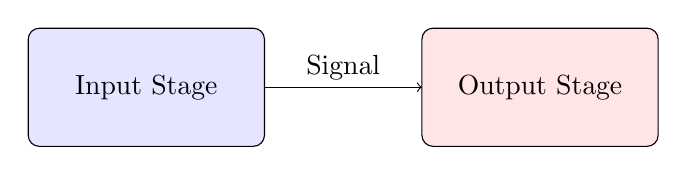
\begin{tikzpicture}
        % Simple block diagram example
        \draw[fill=blue!10, rounded corners] (0,0) rectangle (3,1.5);
        \draw[fill=red!10, rounded corners] (5,0) rectangle (8,1.5);
        \draw[->] (3,0.75) -- (5,0.75);
        
        % Labels
        \node at (1.5,0.75) {Input Stage};
        \node at (6.5,0.75) {Output Stage};
        \node at (4,1) {Signal};
        
    \end{tikzpicture}
    \caption{Example system block diagram}
    \label{fig:example}
\end{figure}

Figure support is built into the class. As shown in \figref{\ref{fig:example}}, you can create diagrams using TikZ and reference them with the \texttt{\\figref} command. The class also provides support for SI units through the siunitx package: \SI{12.5}{\milli\second}.

% Feature 10: Problems Encountered section
\reportProblems
This demonstrates the \texttt{\\reportProblems} command which creates the Problems Encountered section. This section should document challenges encountered during the reporting period and describe steps taken to overcome them.

For example: Initial testing of the sensor network revealed an unacceptable 8\% packet loss rate when multiple nodes transmitted simultaneously. After investigation, I determined the issue stemmed from improper collision avoidance timing. To address this, I implemented a randomized backoff algorithm based on the node ID, which reduced packet loss to below 1\%, within our acceptable performance threshold.

% Feature 11: Plans for Following Period section
\reportPlans
This demonstrates the \texttt{\\reportPlans} command which creates the Plans for Following Period section. This section should outline specific goals and tasks for the next reporting period:

\begin{itemize}
    \item Complete integration of sensor network with the central control system
    \item Optimize power consumption of wireless nodes
    \item Develop automated testing framework for system validation
    \item Document API specifications for other team members
\end{itemize}

% Feature 12: Changes to Requirements section
\reportReqChanges
This demonstrates the \texttt{\\reportReqChanges} command which creates the Changes to Requirements section. This section should document any modifications to project requirements identified during the reporting period.

No changes to the project requirements have been identified during this reporting period. The current specifications remain appropriate for meeting our project goals and timeline.

% Feature 13: Optional Assessment section
\reportAssessment
This demonstrates the \texttt{\\reportAssessment} command which creates the optional Assessment section. This section provides an overall evaluation of project status, including schedule compliance and progress toward milestones.

The project is currently on schedule with all team members making consistent progress. Our weekly coordination meetings have been effective in maintaining alignment between hardware, firmware, and software components. Based on current development velocity, we expect to meet our midterm milestone of delivering a functional prototype by October 15th.

% Feature 14: Optional Instructor Issues section
\reportInstructorIssues
This demonstrates the \texttt{\\reportInstructorIssues} command which creates the optional Instructor Issues section. Use this section to highlight concerns requiring instructor attention or to ask specific questions.

We would appreciate guidance on accessing the RF test equipment in the communications lab for antenna characterization measurements. Our team will need approximately 3 hours of lab time during the week of September 21st.

\newpage

%% ============================================================================
%% CODE ENVIRONMENT WRAPPERS
%% ============================================================================

\textbf{Code Environment Wrappers:}

The capstone\_report class provides specialized environments for displaying code in various programming languages with proper syntax highlighting.

% Feature 15: C/C++ Code Environment
\subhead{C/C++ Code Environment:}

The \texttt{reportcpp} environment displays C and C++ code with proper syntax highlighting:

\begin{reportcpp}[caption=Example C++ Implementation]
#include <iostream>
#include <vector>
#include <cmath>

// Structure to store sensor data
struct SensorReading {
    int id;
    double value;
    double timestamp;
    bool valid;
};

/**
 * Process raw sensor readings and apply filtering
 * @param readings Vector of raw sensor readings
 * @return Vector of filtered readings
 */
std::vector<double> processReadings(const std::vector<SensorReading>& readings) {
    std::vector<double> processed;
    constexpr double THRESHOLD = 0.5;
    
    // Apply moving average filter to valid readings
    for (size_t i = 0; i < readings.size(); i++) {
        if (readings[i].valid && fabs(readings[i].value) > THRESHOLD) {
            processed.push_back(readings[i].value);
        } else {
            processed.push_back(0.0);  // Invalid reading
        }
    }
    
    return processed;
}

// Main processing function
int main() {
    // Sample sensor data
    std::vector<SensorReading> data = {
        {1, 2.5, 0.0, true},
        {2, 3.7, 0.1, true},
        {3, 0.2, 0.2, false},
        {4, 4.1, 0.3, true}
    };
    
    // Process the readings
    auto results = processReadings(data);
    
    // Output results
    std::cout << "Processed Readings:\n";
    for (size_t i = 0; i < results.size(); i++) {
        std::cout << "Sensor " << data[i].id << ": " 
                  << results[i] << "\n";
    }
    
    return 0;
}
\end{reportcpp}

% Feature 16: Python Code Environment
\subhead{Python Code Environment:}

The \texttt{reportpython} environment displays Python code with proper syntax highlighting:

\begin{reportpython}[caption=Data Analysis Example]
#!/usr/bin/env python3
import numpy as np
import matplotlib.pyplot as plt
from scipy.signal import find_peaks

def analyze_sensor_data(filename, threshold=0.75):
    """Analyze sensor readings from a data file
    
    Args:
        filename (str): Path to the data file
        threshold (float): Detection threshold (0-1)
        
    Returns:
        tuple: (peaks, metrics) where peaks are detected events
               and metrics are statistical measures
    """
    # Load data from file
    data = np.loadtxt(filename, delimiter=',')
    time = data[:, 0]
    values = data[:, 1]
    
    # Find peaks in the signal
    peaks, _ = find_peaks(values, height=threshold*np.max(values))
    
    # Calculate metrics
    metrics = {
        'mean': np.mean(values),
        'std_dev': np.std(values),
        'peak_count': len(peaks),
        'max_value': np.max(values)
    }
    
    # Plot the results
    plt.figure(figsize=(10, 6))
    plt.plot(time, values, 'b-')
    plt.plot(time[peaks], values[peaks], 'ro')
    plt.xlabel('Time (s)')
    plt.ylabel('Sensor Value')
    plt.title(f'Sensor Data Analysis - {len(peaks)} peaks detected')
    plt.grid(True)
    plt.savefig('sensor_analysis.png')
    
    return peaks, metrics
    
# Example usage
if __name__ == "__main__":
    peaks, metrics = analyze_sensor_data("sensor_data.csv", 0.6)
    print(f"Found {len(peaks)} peaks")
    print(f"Average value: {metrics['mean']:.2f}")
\end{reportpython}

% Feature 17: MATLAB Code Environment
\subhead{MATLAB Code Environment:}

The \texttt{reportmatlab} environment displays MATLAB code with proper syntax highlighting:

\begin{reportmatlab}[caption=Control System Simulation]
% Control system simulation for energy management
function [response, energy_saved] = simulate_control_system(setpoint, duration)
    % System parameters
    Kp = 2.5;  % Proportional gain
    Ki = 0.8;  % Integral gain
    Kd = 0.4;  % Derivative gain
    
    % Time vector
    dt = 0.01;
    t = 0:dt:duration;
    
    % Initialize variables
    n = length(t);
    response = zeros(1, n);
    error = zeros(1, n);
    control = zeros(1, n);
    
    % External disturbance model (random fluctuations)
    disturbance = 0.2*randn(1, n) + 0.1*sin(0.5*t);
    
    % Simulation loop
    for i = 2:n
        % Calculate error
        error(i) = setpoint - response(i-1);
        
        % PID control
        P = Kp * error(i);
        I = Ki * sum(error(1:i)) * dt;
        D = Kd * (error(i) - error(i-1)) / dt;
        
        % Apply control and system dynamics
        control(i) = P + I + D;
        response(i) = response(i-1) + (control(i) - 0.3*response(i-1) + disturbance(i)) * dt;
    end
    
    % Calculate energy savings compared to no control
    no_control = cumsum(disturbance) * dt;
    energy_saved = sum(abs(no_control) - abs(response)) / sum(abs(no_control)) * 100;
    
    % Plot results
    figure;
    subplot(2, 1, 1);
    plot(t, response, 'b-', t, setpoint*ones(1, n), 'r--');
    legend('System Response', 'Setpoint');
    xlabel('Time (s)');
    ylabel('Temperature (C)');
    title('Smart Energy Control Simulation');
    
    subplot(2, 1, 2);
    plot(t, control, 'g-');
    xlabel('Time (s)');
    ylabel('Control Signal');
    
    fprintf('Energy saved: %.2f%%\n', energy_saved);
end
\end{reportmatlab}

% Feature 18: Terminal Output Environment
\subhead{Terminal Output Environment:}

The \texttt{reportterminal} environment displays terminal commands and outputs with proper styling:

\begin{reportterminal}[caption=Building and Flashing the Firmware]
$ cd ~/projects/smart-energy-system
$ make clean
rm -f build/*.o build/*.elf build/*.bin build/*.hex
$ make
Compiling src/main.c
Compiling src/sensor_protocol.c
Compiling src/backoff.c
Compiling src/uart.c
Compiling src/crc16.c
Linking build/firmware.elf
Creating build/firmware.bin
Creating build/firmware.hex

Build successful!
  text    data     bss     dec     hex
 25460    1024    3620   30104    7588

$ make flash
Flashing device using ST-Link...
Erasing memory
Programming 26484 bytes...
Verification successful
Resetting device...
$ make monitor
--- Terminal connected to /dev/ttyUSB0 (115200,8,N,1) ---
[INFO] Smart Energy System Firmware v1.2
[INFO] Initializing hardware...
[INFO] Sensor network started, 5 nodes detected
[INFO] Energy monitoring active
[DATA] Temperature: 23.5C, Humidity: 42%
[DATA] Current consumption: 120.3 mA
^C
Terminal closed
\end{reportterminal}

% Feature 19: Appendix Support
\reportappendix{Additional Materials}

The \texttt{\\reportappendix} command creates an appendix with an optional title. This is useful for including supplementary materials that would interrupt the flow of the main report.

This appendix demonstrates how to include detailed calculations, reference materials, or additional code listings that support the main report content but are not essential to understanding the primary progress made during the reporting period.

\begin{reportcpp}[caption=Full Protocol Implementation]
/* Complete protocol implementation example */
#include "protocol.h"

/* Initialize protocol with specified parameters */
bool protocol_init(uint8_t address, uint32_t baudrate) {
    /* Configure hardware */
    uart_config_t config = {
        .baudrate = baudrate,
        .data_bits = 8,
        .parity = UART_PARITY_NONE,
        .stop_bits = 1
    };
    
    /* Initialize UART hardware */
    if (!uart_initialize(&config)) {
        return false;
    }
    
    /* Set node address in internal state */
    g_node_address = address;
    
    /* Initialize collision avoidance system */
    backoff_init(address);
    
    return true;
}

/* Send data packet with error checking */
bool protocol_send(const uint8_t* data, uint8_t length) {
    /* Create packet */
    Packet packet;
    packet.header = PROTOCOL_MAGIC;
    packet.address = g_node_address;
    packet.type = PACKET_TYPE_DATA;
    
    /* Implement collision avoidance */
    uint32_t backoff = calculate_random_backoff();
    delay_microseconds(backoff);
    
    /* Transmit packet */
    uart_write(&packet, sizeof(Packet));
    uart_write(data, length);
    
    /* Add CRC-16 for error detection */
    uint16_t crc = calculate_crc16(data, length);
    uart_write(&crc, sizeof(uint16_t));
    
    return true;
}

/* Receive data with timeout */
bool protocol_receive(uint8_t* buffer, uint8_t max_len, uint32_t timeout) {
    /* Wait for packet header */
    Packet packet;
    uint32_t start_time = get_system_time();
    bool timeout_occurred = false;
    
    /* Timeout loop */
    while (!uart_data_available() && !timeout_occurred) {
        if ((get_system_time() - start_time) > timeout) {
            timeout_occurred = true;
        }
        yield_cpu();
    }
    
    if (timeout_occurred) {
        return false;
    }
    
    /* Read packet header */
    uart_read(&packet, sizeof(Packet));
    
    /* Validate packet */
    if (packet.header != PROTOCOL_MAGIC) {
        return false;  /* Invalid magic number */
    }
    
    /* Check if packet is for us */
    if (packet.address != g_node_address && packet.address != BROADCAST_ADDRESS) {
        return false;  /* Not for us */
    }
    
    /* Read data */
    uint8_t len = min(packet.length, max_len);
    uart_read(buffer, len);
    
    /* Verify CRC */
    uint16_t received_crc;
    uart_read(&received_crc, sizeof(uint16_t));
    uint16_t calculated_crc = calculate_crc16(buffer, len);
    
    return (received_crc == calculated_crc);
}
\end{reportcpp}

\reportappendix{Testing Results}

This second appendix demonstrates that multiple appendices are supported. Notice that appendices are lettered automatically (Appendix A, Appendix B, etc.).

\begin{table}[h]
    \centering
    \begin{tabular}{|c|c|c|c|}
        \hline
        \textbf{Test Case} & \textbf{Input} & \textbf{Expected Output} & \textbf{Result} \\
        \hline
        TC-001 & 5V, 100mA & 4.95-5.05V & PASS \\
        TC-002 & 5V, 500mA & 4.90-5.10V & PASS \\
        TC-003 & 3.3V, 100mA & 3.25-3.35V & PASS \\
        TC-004 & 3.3V, 300mA & 3.20-3.40V & FAIL \\
        \hline
    \end{tabular}
    \caption{Voltage Regulation Test Results}
    \label{tab:voltage-tests}
\end{table}

\end{document}